%%%%%%%%%%%%%%%%%%%%%%%%%%%%%%%%%%%%%%%%%
% Lachaise Assignment
% LaTeX Template
% Version 1.0 (26/6/2018)
%
% This template originates from:
% http://www.LaTeXTemplates.com
%
% Authors:
% Marion Lachaise & François Févotte
% Vel (vel@LaTeXTemplates.com)
%
% License:
% CC BY-NC-SA 3.0 (http://creativecommons.org/licenses/by-nc-sa/3.0/)
% 
%%%%%%%%%%%%%%%%%%%%%%%%%%%%%%%%%%%%%%%%%

%----------------------------------------------------------------------------------------
%	PACKAGES AND OTHER DOCUMENT CONFIGURATIONS
%----------------------------------------------------------------------------------------

\documentclass[12pt]{article}
\usepackage{graphicx}
\usepackage{amsmath}
\usepackage{fontawesome5}
\usepackage{booktabs}
\usepackage{amssymb}
\usepackage{hyperref}
\usepackage{amsthm}
\usepackage{newpxtext}
\usepackage[toc,page]{appendix}
\usepackage[nottoc]{tocbibind}
\numberwithin{equation}{section}
\graphicspath{ {./Images/} }
\usepackage[raggedright]{titlesec}
\usepackage{placeins}
%%%%%%%%%%%%%%%%%%%%%%%%%%%%%%%%%%%%%%%%%
% Lachaise Assignment
% Structure Specification File
% Version 1.0 (26/6/2018)
%
% This template originates from:
% http://www.LaTeXTemplates.com
%
% Authors:
% Marion Lachaise & François Févotte
% Vel (vel@LaTeXTemplates.com)
%
% License:
% CC BY-NC-SA 3.0 (http://creativecommons.org/licenses/by-nc-sa/3.0/)
% 
%%%%%%%%%%%%%%%%%%%%%%%%%%%%%%%%%%%%%%%%%

%----------------------------------------------------------------------------------------
%	PACKAGES AND OTHER DOCUMENT CONFIGURATIONS
%----------------------------------------------------------------------------------------

\usepackage{amsmath,amsfonts,stmaryrd,amssymb} % Math packages

\usepackage{enumerate} % Custom item numbers for enumerations

\usepackage[ruled]{algorithm2e} % Algorithms

\usepackage[framemethod=tikz]{mdframed} % Allows defining custom boxed/framed environments

\usepackage{listings} % File listings, with syntax highlighting
\lstset{
	basicstyle=\ttfamily, % Typeset listings in monospace font
}

%----------------------------------------------------------------------------------------
%	DOCUMENT MARGINS
%----------------------------------------------------------------------------------------

\usepackage{geometry} % Required for adjusting page dimensions and margins

\geometry{
	paper=a4paper, % Paper size, change to letterpaper for US letter size
	top=3.81cm, % Top margin
	bottom=3.81cm, % Bottom margin
	left=3.81cm, % Left margin
	right=3.81cm, % Right margin
	headheight=14pt, % Header height
	footskip=1.5cm, % Space from the bottom margin to the baseline of the footer
	headsep=1.2cm, % Space from the top margin to the baseline of the header
	%showframe, % Uncomment to show how the type block is set on the page
}

%----------------------------------------------------------------------------------------
%	FONTS
%----------------------------------------------------------------------------------------

\usepackage[utf8]{inputenc} % Required for inputting international characters
\usepackage[T1]{fontenc} % Output font encoding for international characters


\mdfdefinestyle{commandline}{
	leftmargin=10pt,
	rightmargin=10pt,
	innerleftmargin=15pt,
	middlelinecolor=black!50!white,
	middlelinewidth=2pt,
	frametitlerule=false,
	backgroundcolor=black!5!white,
	frametitle={Command Line},
	frametitlefont={\normalfont\sffamily\color{white}\hspace{-1em}},
	frametitlebackgroundcolor=black!50!white,
	nobreak,
}

% Define a custom environment for command-line snapshots
\newenvironment{commandline}{
	\medskip
	\begin{mdframed}[style=commandline]
}{
	\end{mdframed}
	\medskip
}

%----------------------------------------------------------------------------------------
%	FILE CONTENTS ENVIRONMENT
%----------------------------------------------------------------------------------------

% Usage:
% \begin{file}[optional filename, defaults to "File"]
%	File contents, for example, with a listings environment
% \end{file}

\mdfdefinestyle{file}{
	innertopmargin=1.6\baselineskip,
	innerbottommargin=0.8\baselineskip,
	topline=false, bottomline=false,
	leftline=false, rightline=false,
	leftmargin=2cm,
	rightmargin=2cm,
	singleextra={%
		\draw[fill=black!10!white](P)++(0,-1.2em)rectangle(P-|O);
		\node[anchor=north west]
		at(P-|O){\ttfamily\mdfilename};
		%
		\def\l{3em}
		\draw(O-|P)++(-\l,0)--++(\l,\l)--(P)--(P-|O)--(O)--cycle;
		\draw(O-|P)++(-\l,0)--++(0,\l)--++(\l,0);
	},
	nobreak,
}

% Define a custom environment for file contents
\newenvironment{file}[1][File]{ % Set the default filename to "File"
	\medskip
	\newcommand{\mdfilename}{#1}
	\begin{mdframed}[style=file]
}{
	\end{mdframed}
	\medskip
}

%----------------------------------------------------------------------------------------
%	NUMBERED QUESTIONS ENVIRONMENT
%----------------------------------------------------------------------------------------

% Usage:
% \begin{question}[optional title]
% Question contents
% \end{question}

\mdfdefinestyle{question}{
	innertopmargin=1.2\baselineskip,
	innerbottommargin=0.8\baselineskip,
	roundcorner=5pt,
	nobreak,
	singleextra={%
		\draw(P-|O)node[xshift=1em,anchor=west,fill=white,draw,rounded corners=5pt]{%
		\theQuestion\questionTitle};
	},
}


% Define a custom environment for numbered questions
\newenvironment{question}[1][\unskip]{
	\bigskip
	\stepcounter{Question}
	\newcommand{\questionTitle}{~#1}
	\begin{mdframed}[style=question]
}{
	\end{mdframed}
	\medskip
}

%----------------------------------------------------------------------------------------
%	WARNING TEXT ENVIRONMENT
%----------------------------------------------------------------------------------------

% Usage:
% \begin{warn}[optional title, defaults to "Warning:"]
%	Contents
% \end{warn}

\mdfdefinestyle{warning}{
	topline=false, bottomline=false,
	leftline=false, rightline=false,
	nobreak,
	singleextra={%
		\draw(P-|O)++(-0.7em,0)node(tmp1){};
		\draw(P-|O)++(0.7em,0)node(tmp2){};
		\fill[white,rotate around={45:(P-|O)}](tmp1)rectangle(tmp2);
		\node at(P-|O){\color{black}\scriptsize\bf};
		\draw[very thick](P-|O)++(0,-1em)--(O);%--(O-|P);
	}
}

% Define a custom environment for warning text
\newenvironment{warn}[1][Warning:]{ % Set the default warning to "Warning:"
	\medskip
	\begin{mdframed}[style=warning]
		\noindent{\textbf{#1}}
}{
	\end{mdframed}
}

%----------------------------------------------------------------------------------------
%	INFORMATION ENVIRONMENT
%----------------------------------------------------------------------------------------

% Usage:
% \begin{info}[optional title, defaults to "Info:"]
% 	contents
% 	\end{info}

\mdfdefinestyle{info}{%
	topline=false, bottomline=false,
	leftline=false, rightline=false,
	nobreak,
	singleextra={%
		\fill[black](P-|O)circle[radius=0.4em];
		\node at(P-|O){\color{white}\scriptsize\bf i};
		\draw[very thick](P-|O)++(0,-0.8em)--(O);%--(O-|P);
	}
}

% Define a custom environment for information
\newenvironment{info}[1][Info:]{ % Set the default title to "Info:"
	\medskip
	\begin{mdframed}[style=info]
		\noindent{\textbf{#1}}
}{
	\end{mdframed}
}
\newcommand\specpar[1]{%
  \edef\svparindent{\the\parindent}%
  \setbox0=\hbox{\parbox[t]{\dimexpr\textwidth-6pt}{\strut\hspace{\svparindent}#1\strut}}%
  \par%
  \noindent\textcolor{gray}{\rule[-\dp0]{2pt}{\dimexpr\dp0+\ht0}}\kern4pt\copy0%
  \par%
}
\usepackage{mathtools}
\newcommand\numberthis{\addtocounter{equation}{1}\tag{\theequation}}
\newcommand{\QED}{\tag*{$\square$}}
\newtheorem{theorem}{Theorem}[section]
\newtheorem{corollary}{Corollary}[theorem]
\newtheorem{lemma}[theorem]{Lemma}
\interfootnotelinepenalty=10000
\makeatletter

\newcommand\frontmatter{%
    \cleardoublepage
  %\@mainmatterfalse
  \pagenumbering{roman}}

\newcommand\mainmatter{%
    \cleardoublepage
 % \@mainmattertrue
  \pagenumbering{arabic}}


\makeatother

\title{Calculating mathematical constants \\with Monte Carlo simulations}

\author{Bhoris Dhanjal\\ Khushi Chauhan }

\date{\today} 
\newcommand{\reporttitle}{{Calculating mathematical constants with  Monte Carlo\\[0.15in] simulations}}


%----------------------------------------------------------------------------------------

\begin{document}
% Last modification: 2015-08-17 (Marc Deisenroth)
\begin{titlepage}

\newcommand{\HRule}{\rule{\linewidth}{0.5mm}} % Defines a new command for the horizontal lines, change thickness here




\center % Center remainder of the page

%----------------------------------------------------------------------------------------
%	HEADING SECTIONS
%----------------------------------------------------------------------------------------
\begin{center}
    



%----------------------------------------------------------------------------------------
%	TITLE SECTION
%----------------------------------------------------------------------------------------

\includegraphics[width=0.2\textwidth]{Images/xavierslogo.png}\\[1.5cm]
\HRule \\[0.4cm]
{ \huge \bfseries \reporttitle}\\[0.4cm] % Title of your document
\HRule \\[2.5cm]
\end{center}
%----------------------------------------------------------------------------------------
%	AUTHOR SECTION
%----------------------------------------------------------------------------------------
\textbf{
\large A project submitted to\\
\large Department of Statistics\\
\large St. Xavier’s College (Autonomous), Mumbai\\
\large by\\[1cm]
\large Bhoris Dhanjal\\
Khushi Chauhan}

%----------------------------------------------------------------------------------------
%	FOOTER & DATE SECTION
%----------------------------------------------------------------------------------------
\vfill % Fill the rest of the page with whitespace
\textbf{
2020-2021}
\end{titlepage}

\frontmatter
\begin{center}
    \large St. Xavier’s College (Autonomous), Mumbai\\
\large Department of Statistics\\
\large Project by\\
\begin{table}[h!]
\centering
\begin{tabular}{ccccc}
\hline
Sr. No. & Name of Student & Class & UID & Roll No. \\ \hline
1 & Bhoris Dhanjal & SYBSc & 202020 & 314 \\
2 & Khushi Chauhan & SYBSc & 202019 & 313 \\ \hline
\end{tabular}
\end{table}
Title of the Project:\\
Calculating mathematical constants with Monte Carlo simulations
\end{center}
\clearpage

\section*{\centering{Declaration by the Student}}
\addcontentsline{toc}{section}{Declaration by the Student}
\par We hereby declare that the project entitled “Calculating mathematical constants with Monte Carlo simulations” was completed and
written by us is the result of original project work and has not formed earlier the basis for
the certificate (any award) or similar title of this or any other school/college or examining
body.
\vfill
Date: \today \par
Name and Signature of Student:\\
\par Bhoris Dhanjal \hfill Khushi Chauhan\\
\clearpage

\section*{\centering{Acknowledgements}}
\addcontentsline{toc}{section}{Acknowledgements}
We would like to express our deepest thanks to our professors, Prof. Myrtle Fernandes and Prof. Ayesha Dias and the rest of the Department of Statistics at St. Xavier's, for encouraging us to explore this topic.
\par We would further like to thank our friends and family for offering emotional support.
\par We further extend our gratitude towards the vast trove of information we gleaned from the internet, via papers and various online forums on StackExchange (CrossValidated, Mathematics, Mathematica \& TeX).
\clearpage
\tableofcontents


%----------------------------------------------------------------------------------------
%	INTRODUCTION
%----------------------------------------------------------------------------------------
\mainmatter
\maketitle
\begin{abstract}
    This project primarily serves to showcase Monte Carlo simulations. We first derive the naïve Monte Carlo estimator for numerical integration. Following which we use Monte Carlo simulations to estimate a few well known mathematical constants. Variance reduction techniques and Quasi-Monte Carlo integration will be examined at the end.
\end{abstract}
\section{Introduction} % Unnumbered section
In this project we will explore Monte Carlo simulations.
The objectives of this project are as follows:
\begin{itemize}
    \item Provide a conceptual overview of the Monte Carlo method.
    \item Describing and demonstrating naïve numerical Monte Carlo integration.
    \item Using various Monte Carlo simulations to calculate $\pi, e, \gamma_n, \phi$, and $\zeta (3)$.
    \item Describing variance reduction techniques for Monte Carlo integration.
    \item Demonstrating Quasi-Monte Carlo integration and comparing it with naïve numerical MC integration.
\end{itemize}\par
The Mathematica notebook (comprising of all code used for computations and plots) and \LaTeX \ source code for this document can be viewed at GitHub with the following link.\\
\href{https://github.com/BhorisDhanjal/reciprocal-multifactorial-constants}{\faGithubSquare} \href{https://github.com/BhorisDhanjal/MonteCarloMathsConstants}{https://github.com/BhorisDhanjal/MonteCarloMathsConstants}
\vfill
%----------------------------------------------------------------------------------------
%	Section 2
%----------------------------------------------------------------------------------------
\section{Numerical Monte Carlo integration}
In this section we will describe the algorithm for numerical Monte Carlo integration. Before this we will provide a short overview of the concept of Monte Carlo simulations.
\subsection{Overview of Monte Carlo method}
Monte Carlo simulations are a general class of computational algorithms that rely on random number sampling \footnote{Note that for the majority of this project we will be utilizing pseudo-random numbers.}. They are used to estimate numerical results for problems for which analytical solutions are either very difficult to obtain or impossible.
\subsection{Naive Monte Carlo integration}
We can demonstrate the theory behind naïve \footnote{We call it "naïve" since it utilizes uniformly distributed random variates, more sophisticated methods are discussed in the last section of this project.} Monte Carlo integration in a simplified manner as below \cite{caflisch_1998, stefanmontecarlo}.
\begin{theorem}
$\frac{1}{N} \sum_{i=1}^N f(X_i)$ is an unbiased estimator for $\int_{[0,1]^s} f(x)\ dx$
\end{theorem}
For points $x={(x_1,x_2, \dots, x_s)}$ consider a function $f(x)$ over the unit hypercube $[0,1]^s$ in $\mathbb{R}^s$.
\begin{align*}
    \mathcal{I}[f]&=\int_{[0,1]^s} f(x)\ dx
    \intertext{The approximation of $\mathcal{I}[f]$ is given by the expectation of $f(X)$ for some uniformly distributed random variable $X \in [0,1]^s$.}
    \mathcal{I}[f]&=E[f(X)]=E
    \intertext{Where an estimation for expectation is given by the sample mean,}
    \widehat{\mathcal{I}} &= \frac{1}{N}\sum_{i=1}^N f(X_i)
\end{align*}
By the Law of Large numbers \cite{stronglaw} we can state that,
\begin{align*}
    \lim_{N \rightarrow \infty} &\frac{1}{N}\sum_{i=1}^N f(X_i)
    \rightarrow \mathcal{I}[f]
    \intertext{Furthermore we can state that $\widehat{\mathcal{I}}$ is an unbiased estimator since $E[\widehat{\mathcal{I}}]=\mathcal{I}[f]$ for all N}
    \intertext{Therefore, we can estimate $\mathcal{I}[f]$ with,}
    \mathcal{I}[f] &\approx \widehat{\mathcal{I}}= \frac{1}{N}\sum_{i=1}^N f(X_i) \QED
\end{align*}
In general, for a function $f(x)$ over any volume $V$ in $\mathbb{R}^n$ we can say \cite{montecarlowolfram},
\begin{align*}
    \mathcal{I}[f]&=\int_V f(x)\ dx \approx V  \frac{1}{N}\sum_{i=1}^N f(X_i) \numberthis
    \intertext{We can simplify the above expression for the case of a one dimensional integral over some closed interval $[a,b]$ where $a,b \in \mathbb{R}^1$ as,}
    \int_a^b f(x)\ dx &\approx (b-a)\frac{1}{N} \sum_{i=1}^N f(X_i) \numberthis \label{eq 2.3}
\end{align*}
\subsection{Error of Naive Monte Carlo integration}
\begin{theorem}
The standard error of the estimator is inversely proportional to the square root of the number of random points chosen.
\end{theorem}
Consider the variance for above described estimator $\widehat{\mathcal{I}}$,
\begin{align*}
    \sigma^2_{\widehat{\mathcal{I}}}&=\sigma^2\left(\frac{1}{N} \sum_{i=1}^N f(X_i) \right)\\
    &=\frac{1}{N^2}\sigma^2 \left( \sum_{i=1}^N f(X_i) \right)
    \intertext{Since $X_i$ are uniform iid r.v., the variance of the sum is equal to the sum of the variance.}
    &=\frac{1}{N^2} \sum_{i=1}^N \sigma^2(f(X_i))\\
    &=\frac{1}{N^2}N \sigma^2_{f(X_{i})}\\
    \sigma^2_{\widehat{\mathcal{I}}}&=\frac{\sigma^2_{f(X_{i})}}{N}\\
    \sigma_{\widehat{\mathcal{I}}}&=\frac{\sigma_{f(X_{i})}}{\sqrt{N}}\\
               \sigma_{\widehat{\mathcal{I}}}&\propto \frac{1}{\sqrt{N}} \QED
\end{align*}
This implies that, in naïve Monte Carlo integration, reducing the error by half requires increasing the number of random points by a factor of 4. \par We will explore variable reduction methods in the last section of this project. For the rest of this project however, we will only utilize naïve Monte Carlo integration that we implement using pseudo-random numbers.
\subsection{An example of naïve Monte Carlo Integration}
In order to better motivate Monte Carlo integration we will provide a simple visualization.\\
\textbf{Example 1.} Estimating $\int_2^5 100 - 8x^2 + x^3\ dx$ with 5 random points.
\par We begin by generating 6 random real numbers between 2 and 5. We will evaluate these points in $f(x)=100-8x^2+x^3$ and plot it.
\begin{figure}[!htb]
    \centering
    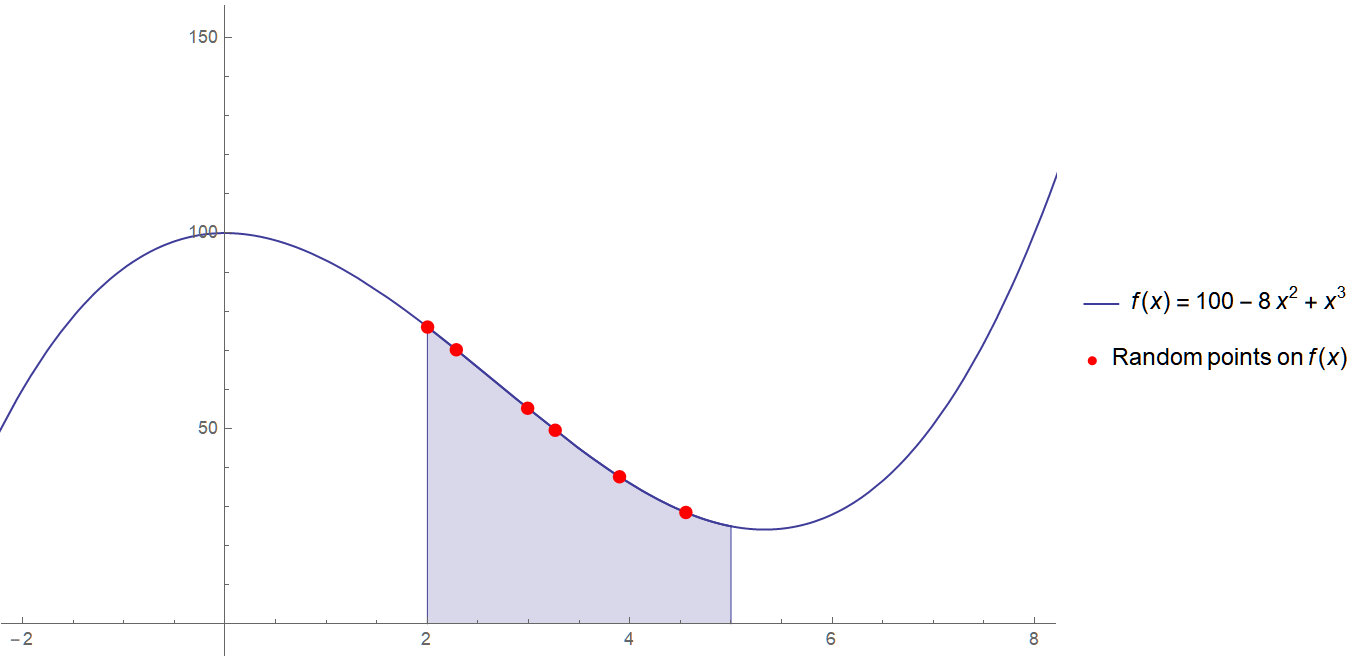
\includegraphics[width=10cm]{Images/pointsexample.png}
    \caption{The plot of f(x) and 6 random points plotted on it.}
    \label{fig:pointsexample}
\end{figure}
\begin{figure}[!htb]
    \centering
    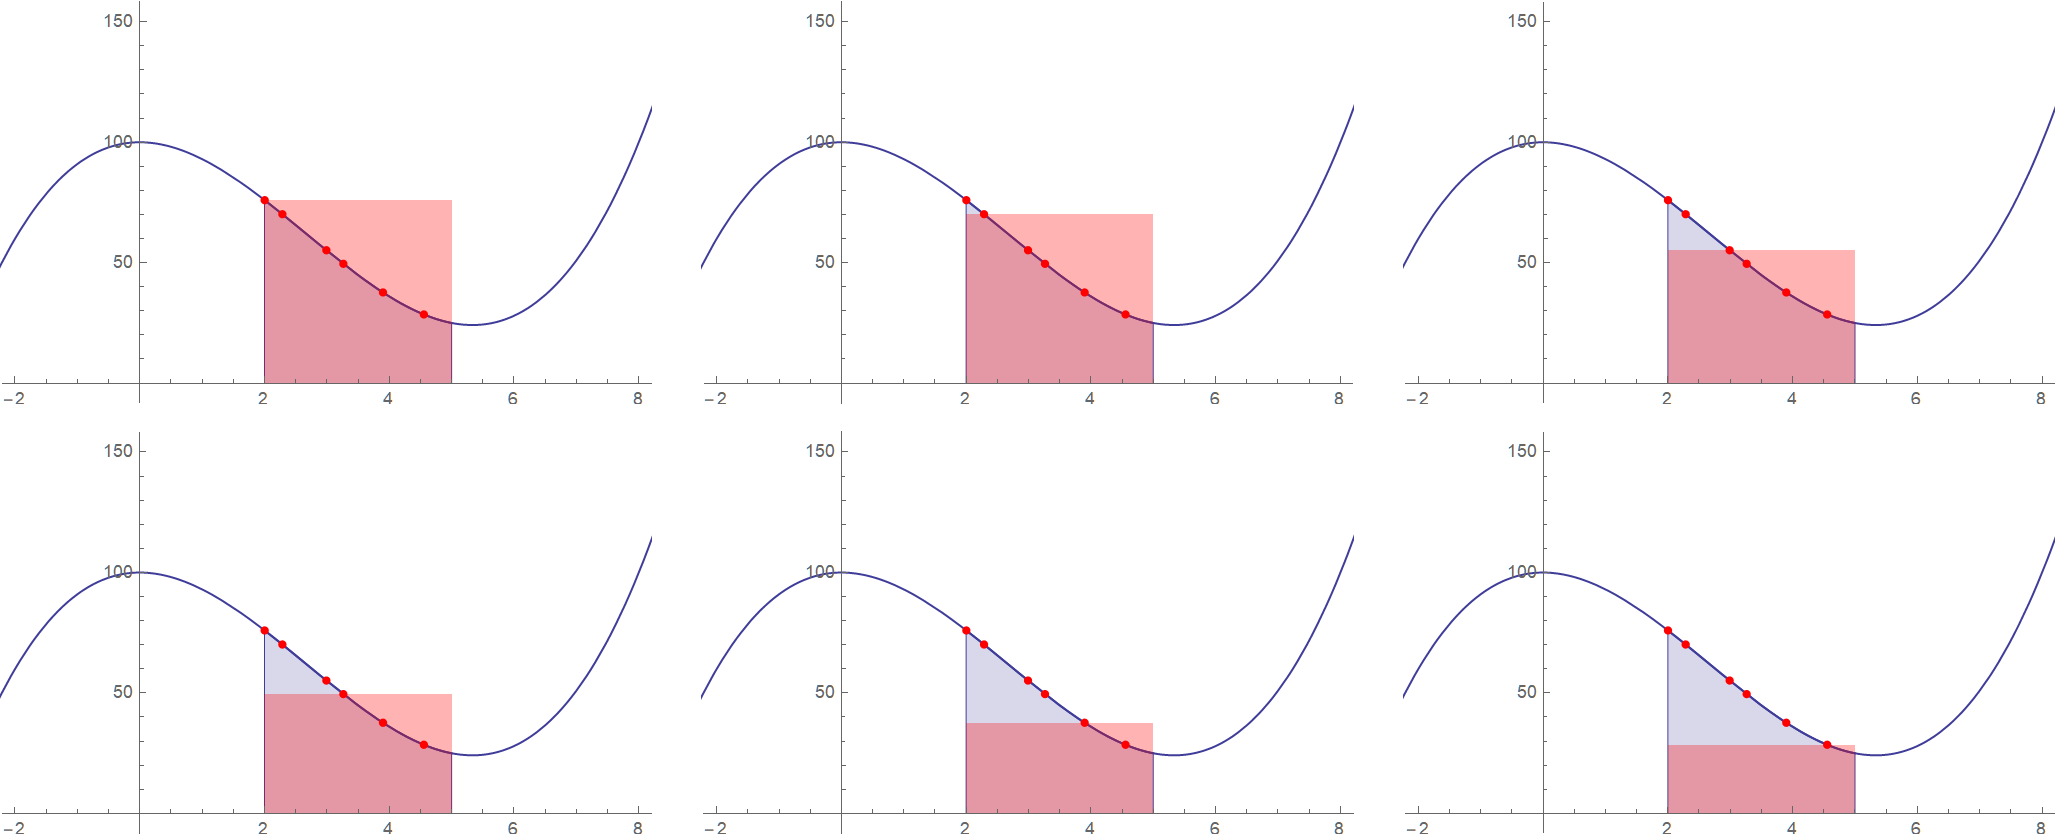
\includegraphics[width=10cm]{Images/rectexample.png}
    \caption{Rectangles of width $(b-a)$ with height corresponding to the random points.}
    \label{fig:rectexample}
\end{figure}\par
Recall eq. \ref{eq 2.3}, the multiplication of the $(b-a)$ term can be visualized as rectangles of width $(b-a)$ as above.
It is now clear to see that taking the mean of these rectangle areas will give us an approximation to the integral that improves with the addition of more points.
\clearpage
%----------------------------------------------------------------------------------------
%	Section 3
%----------------------------------------------------------------------------------------
\section{Estimating Pi}
In this section we will discuss the application of  Monte  Carlo  techniques  for  estimating  the  value  of  pi.

\subsection{Elementary Method}
In order to estimate the value of pi using Monte Carlo simulations we will estimate the area of a unit circle inscribed in a unit square.
\par
The  experiment is  conducted by taking random sample points in the region of the unit square. For  an unbiased estimator of area of the circle it is assumed  that the  random sample  points are uniformly distributed.
\par
The bounding box area is  $A_{box}=r^2=1$ and the area of the unit circle inscribed in the square is $A_{circle}=\pi r^2=\pi$. With $N_{box}$ total sample points and $N_{circle}$ is the total sample points lying inside the unit circle.
\par
Since the sample points are uniformly distributed within the bounding box, the ratio of the circle to the area of the  bounding  box is  approximately  equal  to  the ratio  of the number  of  sample  points  falling  in  the circle to the number of points falling in the bounding box.
\begin{align}
   \frac{A_{pi}}{A_{box}}=\frac{\pi r^2}{r^2}=\pi\approx \frac{N_{pi}}{N_{box}} 
\end{align}
\par An example of a single experiment is shown below.
\begin{figure}[!htb]
    \centering
    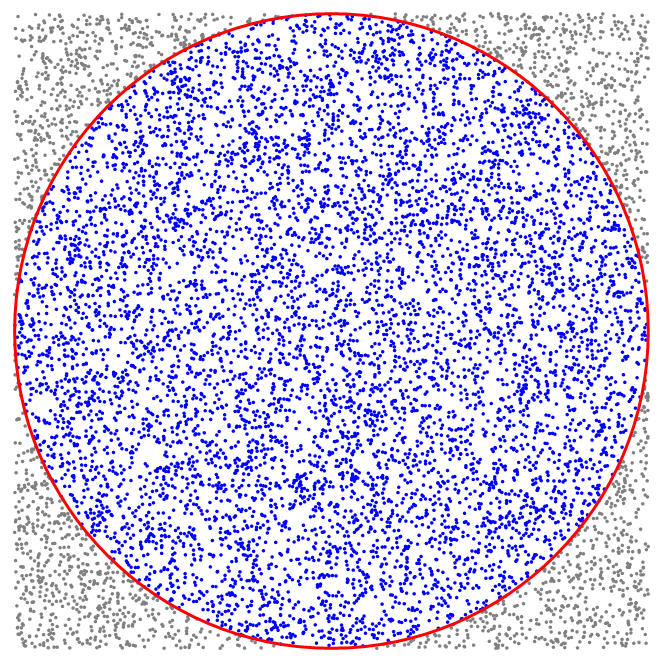
\includegraphics[width=8cm]{Images/piexample.png}
    \caption{Experiment with 10,000 points, $N_{pi}/N_{box}=3.1512$}
    \label{fig:piexample}
\end{figure}\par
We now repeat the experiment $10^3$ times with $10^6$ points. Taking the mean of these $10^3$ experiments gives us the following approximation. $\pi \approx 3.14154 \pm 0.00165$, with $ -1.696 \cdot 10^{-3}\ \%$ error.
\begin{figure}[!htb]
    \centering
    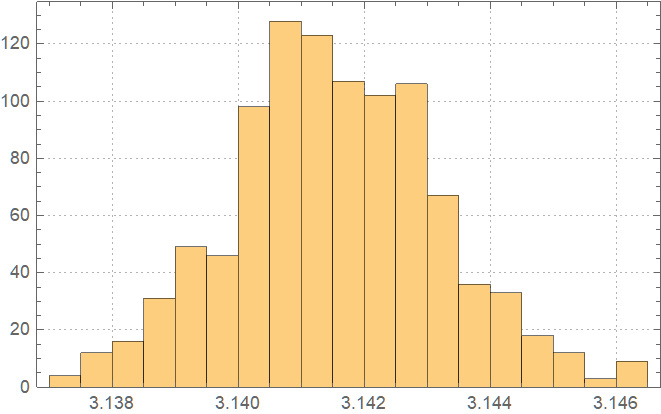
\includegraphics[width=10cm]{Images/repeatedpi.png}
    \caption{Histogram of experiment with $10^6$ points, repeated $10^3$ times.}
    \label{fig:repeatedpi}
\end{figure}

\subsection{Buffon's Needle}
 \textit{“A large plane area is ruled with equidistant parallel lines, the distance between two consecutive lines is 'a'. A thin needle of length $l< a$ is tossed randomly onto the plane. What is the probability that the needle will intersect one of the lines?"}\par
 This forms the basis of the Buffon’s Needle problem. Which can be solved using elementary integral calculus \cite{needlewang}. with the help of this analytical solution, the experiment can be used to approximate $\pi$ using Monte Carlo simulations.
\begin{theorem}
The probability of a needle intersecting a line is given by $p=\frac{2l}{a \pi}$.
\end{theorem}
 For a given needle of length $l$ we model the dropping of the needle on the ruled plane with parallel lines $a$ units apart as follows. \par
 Let x be the distance from the center of the needle to the nearest line and $\theta$ be the acute angle between the needle and the lines. Let x be a uniform random variable over the interval
\par
The uniform probability density function of x between 0 and $ \frac{t}{2}$ is
\[
\begin{cases}
   \dfrac{2}{a} & 0 \leqslant x\leqslant \dfrac{a}{2}\\
  0 & \text {   otherwise}
\end{cases}
\]
\par
and $\theta$ a uniform random variable over the interval $\left(0, \frac{\pi}{2}\right)$ with the probability density function:\\
\[
\begin{cases}
    \dfrac{2}{\pi} & 0 \leqslant x\leqslant \dfrac{\pi}{2}\\
    0 & \text {   otherwise}
\end{cases}
\]
\par
The two random variables, $x$ and $\theta$, are independent  Therefore the joint probability density function of
$(x,\theta)$ 
\[
\begin{cases}
    \dfrac{4}{a\pi} &  0 \leqslant x\leqslant \dfrac{a}{2} \text{ and } 0 \leqslant x\leqslant \dfrac{\pi}{2}\\
0  &  \text {   otherwise}
\end{cases}\]
\\ for the short needle case $\left( l \leqslant a \right)$  A needle
intersects a line if
\begin{align*}
    \left( x \leqslant \frac{l}{2}\sin \theta \right )
\end{align*}
\\
The probability that the needle will intersect a line is

\begin{align*}
p=\int_{0}^\frac{\pi}{2}\int_{0}^{\frac{l}{2} \sin \theta} f(x,\theta)\ dx\ d\theta = \int_{0}^\frac{\pi}{2}\int_{0}^{\frac{l}{2} \sin \theta} \frac{4}{a\pi}\ dx\ d\theta = \frac{2l}{a\pi} 
\end{align*}

\begin{align*}
    p =\frac{2l}{a\pi} \QED
\end{align*}
\par

If experiment has n needles out of which m needles intersect lines, then the value of p can be estimated as
\begin{align}
    \widehat{p}&=\frac{m}{n} \nonumber
    \intertext{$\pi$ can therefore be estimated by}
    \widehat{\pi}&=\frac{2nl}{ma}
\end{align}\par
An example of a single experiment with 1000 needles is shown below.
We then repeat the experiment $10^3$ times with $10^6$ needles. Taking the mean of these $10^3$ experiments gives us the following approximation. $\pi \approx 3.14018 \pm 0.04510$, with $ -4.481 \cdot 10^{-2}\ \%$ error.
\begin{figure}[!htb]
    \centering
    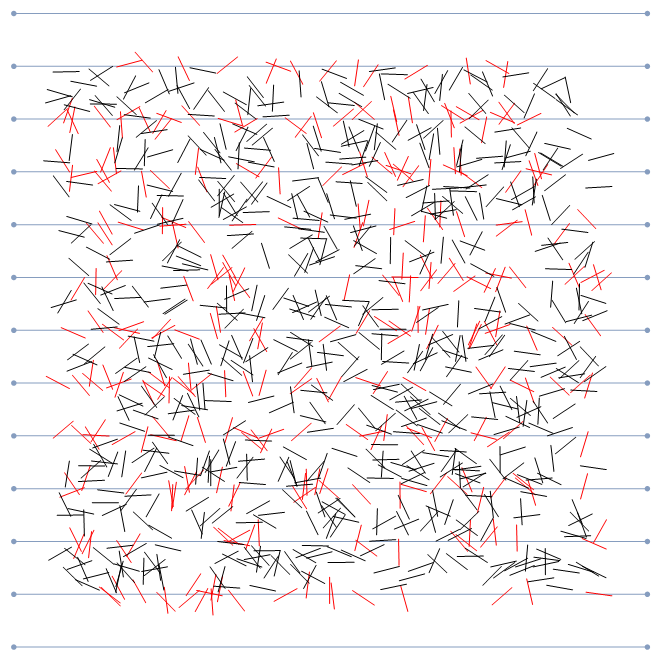
\includegraphics[width=10cm]{Images/needleexample.png}
    \caption{Experiment with 1000 needles, $\widehat{\pi}=3.14465$}
    \label{fig:needleexample}
\end{figure}\par

\begin{figure}[!htb]
    \centering
    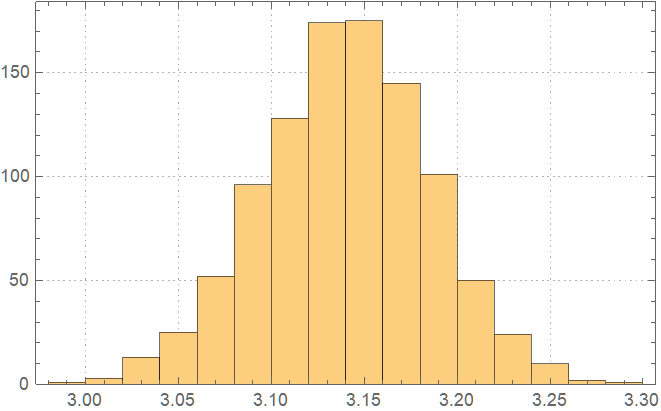
\includegraphics[width=10cm]{Images/repeatedneedle.png}
    \caption{Histogram of Buffon's needle experiment with $10^4$ needles, repeated $10^3$ times.}
    \label{fig:repeatedneedle}
\end{figure}

\clearpage
\subsection{Buffon's Noodle}
Buffon's noodle poses the question, "What is the expected number of crossings if we don't drop a rigid needle but rather a flexible noodle?". In this section we will estimate $\pi$ using Buffon's noodle problem.\par       
For  straight needle $N$  there are  $n$ line crossing for  $n$ intersection of needles with the infinite grid and thus the expectation of line crossing as $E[N]=\frac{2a}{\pi d}$. where $a$ is the length of needle. Using the corollary of this result, that $E[N]$ is a function of the length of the needle
only, not its shape \cite{noodle}.
\begin{theorem}
Let N be a noodle of length 't' thrown at random onto an infinite
grid of parallel lines with common distance d between them. Then the expected number of line-crossings E[N] is given by E[N] = $\frac{2t}{\pi d}$. 
\end{theorem}
\par
We take into consideration the fact that, a noodle due to its shape could cross a line in more than one spot.
In general if a needle intersects $n$ times in $m$ attempts, then a combination of $a$ such needles is expected to be intersected $na$ times in $m$ attempts.
\par 
If this combination is formed by infinitesimally  small needles , then it will become equivalent to a noodle.\par
Consider a sequence of polygonal lines $L_1$  $L_2$,$\cdots$ which approaches the curve of the noodle $N$ uniformly.  Let $L_{i1}$, $L_{i2}$, · · · , $L_{im}$ be the segments of the line $L_i$,
such that $L_i=L_{i1}+L_{i2}+ \cdots +L_{im} $. Let $t_{ij}$ be the length of $L_{ij}$ such that $t_{ij}<d$ for all $i$ and $j$. 
\par
The expectation of line crossing the grid be E[$L_{ij}$] hence
 E[$L_{ij}$] =$ 2t/\pi d$ Now letting $t_i$
be the length of $L_i$, we know that $t_i$ approaches $t$ as $i$ tends to infinity. Hence,
if $E[L_i] = E[L_j] + \cdots +E[L_n] $for all i, then 
\begin{align}
    E[L_i] = \sum_{i=j}^n \frac{2t_{i}}{\pi d} &= \frac{2}{\pi d} \sum_{i=j}^n t_{i} = \frac{2 t}{\pi d}
\intertext{hence in the limit}
E[N]&= \frac{2t}{\pi d} \QED
\end{align}


\subsubsection{A note on the simulation of noodles}
Simulating a "noodle" isn't a very straightforward task computationally, since "noodles" aren't very well defined. Here, we choose to simulate it by considering a line of length $l$ divided into a random number of segments (between 5 and 10), and then randomizing the angles between the segments. One could also choose the make smooth noodles, by using bezier curves instead.
\par 
An example of a single experiment with 1000 noodles is shown  below.\
We now repeat the experiment $250$ times with $10^4$ noodles. Taking the mean of these $250$ experiments gives us the following approximation. $\pi \approx 3.18615 \pm 0.04602$, with a $ + 1.418\ \%$ error.
\begin{figure}[!htb]
    \centering
    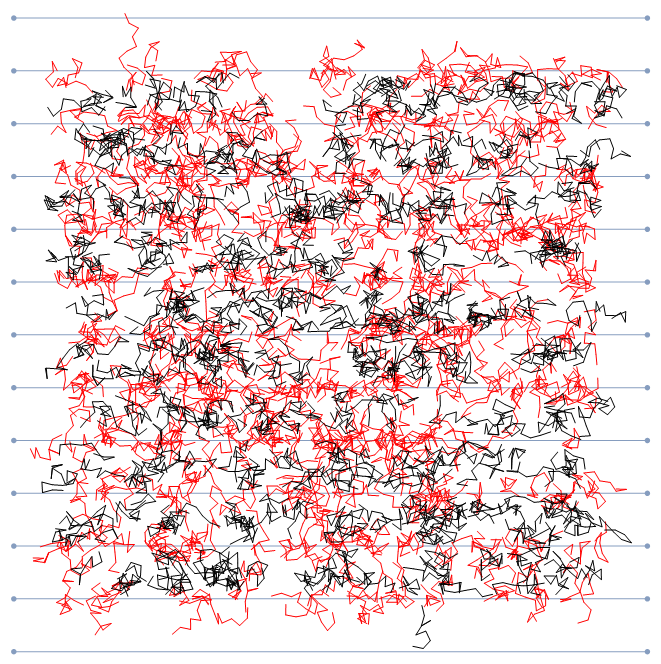
\includegraphics[width=10cm]{Images/noodleexample.png}
    \caption{Experiment with 1000 noodles, $\widehat{\pi}=3.36984$}
    \label{fig:noodleexample}
\end{figure}\par

\begin{figure}[!htb]
    \centering
    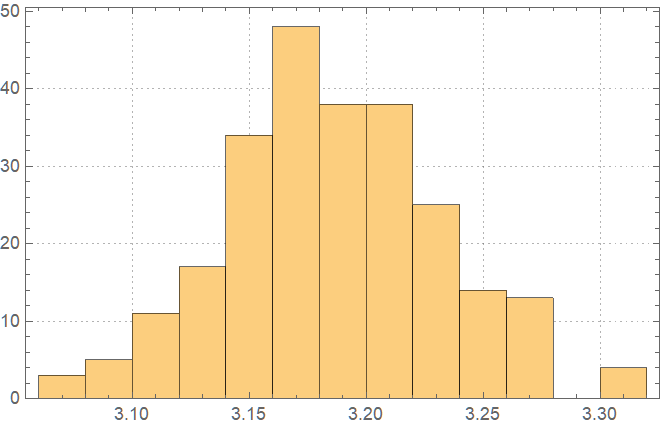
\includegraphics[width=8cm]{Images/repeatednoodle.png}
    \caption{Histogram of Buffon's noodle experiment with $10^4$ needles, repeated $250$ times.}
    \label{fig:repeatednoodle}
\end{figure}
\clearpage
%----------------------------------------------------------------------------------------
%	Section 4
%----------------------------------------------------------------------------------------
\section{Estimating Euler's number}
If $U_1, U_2 \cdots U_n$ are some independent and uniformly distributed random variables over (0,1). Let $S_n=\sum_{i=1}^n U_i$ and if $N$ is the minimum value of $n$ for which $S_n>1$. The expectation of N is in fact equal to $e$.
\par This problem originated from as a exercise from a famous Russian textbook by Gnedenko \cite{gnedenko}. For this section we will be drawing from two papers written by K. G. Russel on this topic \cite{simplerussell, russell_1983}.
\begin{theorem}
For iid uniform r.v. $U_1, U_2 \cdots U_n$ over (0,1), with $S_n=\sum_{i=1}^n U_i$ and if $N$ is the minimum value of $n$ for which $S_n>1$, then $E[N]=e$.
\end{theorem}
    Note that our goal is to show that 
\begin{align}   
    E[N]=\sum_{n=2}^{\infty}n P(N=n) = e
\end{align}
% Attempt 1
% If we can show that $P(N=n)=\frac{n-1}{n!}$, then we are done. Hence we continue as follows,
% \begin{align*}
%     P(N=n)&=P(S_{n}>1 \wedge S_{n-1}<1)\\
%     &=P(S_n>1)P(S_{n-1}<1)=P(S_{n-1}<1)-P(S_{n}<1)
% \end{align*}
% We have further simplified our problem, now all that remains is to find $P(S_n<1).$ We shall prove that $P(S_n<1)=1/n!$ using induction.\\
% Base case n=1,
% \begin{align*}
%     P(S_1 < 1) &= 1 = \frac{1}{1!}
%     \intertext{Assume it holds true for n, consider n+1}
%     P(S_{n+1} < 1) &= P(S_{n}<1) P(U_{n+1}<1-S_n)
%     \intertext{Assume $S_n=m$ for some $m \in (0, 1)$????}
%     &=P(S_n<1) P(U_{n+1}<1-m)\\
%     &=P(S_n<1) (1-m)\\
%     \intertext{If $m=n/(n+1)$ then we are done}
% \end{align*}
% % Attempt 2 
% If we can show that $P(N=n)=\frac{n-1}{n!}$, then we are done. Hence we continue as follows,
% \begin{align*}
%     P(N=n)&=P(S_{n}>1 \wedge S_{n-1}<1)\\
%     &=P(S_n>1)P(S_{n-1}<1)=P(S_{n-1}<1)-P(S_{n}<1)
% \end{align*}
% We have further simplified our problem, now all that remains is to find $P(S_n<1).$ We shall prove that $P(S_n<1)=1/n!$ using induction.\\
% Base case n=1,
% \begin{align*}
%     P(S_1 < 1) &= 1 = \frac{1}{1!}
%     \intertext{Assume it holds true for n.}
%     \intertext{Denote $P(S_n<1)$ as $F_{n}(1)$ and $P(x<1)$ for some $U_i$ as $F(1)$. Consider now the convolution of these two functions. We have to prove the following,}
%     F_{n} \textasteriskcentered F &= \frac{1}{(n+1)!}\\
%     F_{n} \textasteriskcentered F &= \frac{d}{ds}\left. \left( \int_{\mathbb{R}}F_{n, 1}(x, s-x) \right) \right|_{s=1}
% \end{align*}
If we can show that $P(N=n)=\frac{n-1}{n!}$, then we are done. Hence we continue as follows,
\begin{align*}
    P(N=n)&=P(S_{n}>1 \cap S_{n-1}<1)\\
    &=P(S_{n-1}<1)-P(S_{n}<1)
\end{align*}
We have further simplified our problem, now all that remains is to show that $P(S_n<1)=\frac{1}{n!}$. This would complete the proof. We use the CDF of the Irwin-Hall distribution \cite{hall}.
\par The Irwin-Hall distribution is defined as, the sum of n independent and identically distributed, uniform distributions on the unit interval. The CDF of Irwin-Hall distribution is given as \footnote{This can be derived by integrating the pdf, which is in turn derived by induction by taking the convolution of $f_n \ast f$ to prove the $n+1^{th}$ case.}, 
\begin{align*}
    F(x)&=\frac{1}{n!} \sum_{k=0}^{\lfloor x \rfloor} (-1)^k \binom{n}{k} (x-k)^n
    \intertext{For x=1}
    F(1)=P(S_n<1)&=\frac{1}{n!} \sum_{k=0}^{1} (-1)^k \binom{n}{k} (1-k)^n=\frac{1}{n!} \QED 
\end{align*}
\par The astute reader may ask what is $E[N]$ if we consider $S_n>a$ for any real number $a$? This general form is answered in the paper by Russell \cite{russell_1983}.
\par We now continue with the simulation to predict $e$ by choosing $10^6$ random uniform numbers between (0,1) and counting the average number of times it takes for the sum to cross 1.
\par We now repeat the experiment $10^4$ times with $10^6$ numbers per experiment. Taking the mean of these $10^4$ experiments gives us the following approximation. $e \approx 2.71827 \pm 0.00087$, with $ - 3.405 \cdot 10^{-4}\ \%$ error.
\begin{figure}[!htb]
    \centering
    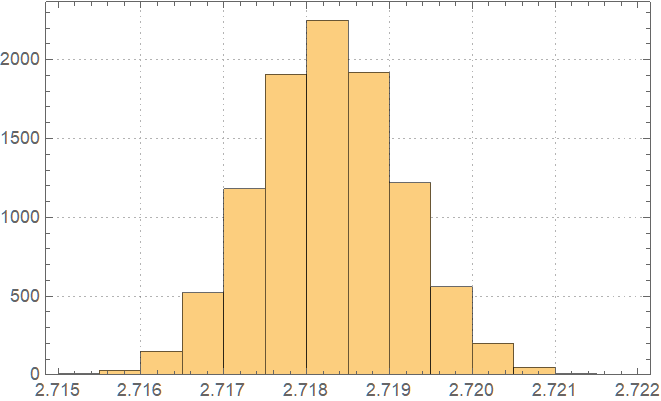
\includegraphics[width=10cm]{Images/repeatede.png}
    \caption{Histogram of $e$ experiment with $10^6$ numbers, repeated $10^4$ times.}
    \label{fig:repeatede}
\end{figure}
%----------------------------------------------------------------------------------------
%	Section 5
%----------------------------------------------------------------------------------------
\section{Estimating Euler-Mascheroni constant and Stieltjes constants}
We begin this section by defining the Euler-Mascheroni constant and Stieltjes constants.
\par The Euler Mascheroni Constant ($\gamma$) is defined as the limiting difference between the harmonic series and the natural logarithm, i.e.
\begin{align}
    \gamma &= \lim_{n \rightarrow \infty} \left( H_n - \log n \right)\\ \label{emconstant}
    &= \lim_{n \rightarrow \infty} \left(\sum_{k=1}^{n} \frac{1}{k} - \log n \right) \nonumber
\end{align}
\par Stieltjes constants can be thought of as a generalization of the Euler-Mascheroni constant, defined as,
\begin{align}
    \gamma_n &= \lim_{m \rightarrow \infty} \left( \sum_{k=1}^m \frac{(\log k)^n}{k} - \frac{(\log m)^{n+1})}{n+1} \right)
\end{align}
\par It is clear to see that $\gamma_0=\gamma$. It is interesting to note that Stieltjes constants were originally discovered in the Laurent series expansion (about 1) of the Riemann Zeta function \cite{stieltjeswolfram}.
\begin{align*}
    \zeta (z) = \frac{1}{z-1} + \sum_{n=0}^\infty \frac{(-1)^n }{n!} \gamma_n (z-1)^n
\end{align*}
We can in fact further generalize Stieltjes constants by considering the Laurent series of the Hurwitz-Zeta function instead of Riemann zeta. However, we will not further examine this.
\subsection{Euler-Mascheroni constant}
% We will first approximate $\gamma$ by using an integral representations of $\gamma$.\par
% We proceed by using the following two known integral representations of $H_n$ and $\log(n)$ in eq \ref{emconstant}.
% \begin{align*}
%     H_n &= \int_0^1 \frac{1-x^n}{1-x}\ dx\\
%     \log n &= \int_0^1 \frac{x^{n-1}-1}{\log x}\ dx
% \end{align*}
% \begin{theorem}
% $\gamma = \int_0^1 \frac{1}{1-x} + \frac{1}{\log x}\ dx$ 
% \end{theorem}
% \begin{align*}
%     \gamma &= \lim_{n \rightarrow \infty} (H_n - \log n)\\
%     &= \lim_{n \rightarrow \infty} \int_0^1 \left( \frac{1-x^n}{1-x} - \frac{x^{n-1}-1}{\log x}\ dx \right)
%     \intertext{Since the function inside the integral is uniformly convergent and bounded, by the Bounded Convergence Theorem we have,}
%     &= \int_0^1 \lim_{n \rightarrow \infty} \left( \frac{1-x^n}{1-x} - \frac{x^{n-1}-1}{\log x} \right)\ dx\\
%     &= \int_0^1 \frac{1}{1-x}+\frac{1}{\log x}\ dx
% \end{align*}
We will estimate the Euler-Mascheroni constant by first approximating the Gumbel distribution \cite{gumbelwolfram}.\par
The Gumbel distribution accepts two parameters, $\alpha$ and $\beta$. It is defined by the following probability density function,
\begin{align*}
    P(x)&=\frac{1}{\beta} e^{\frac{x-\alpha}{\beta}-e^{\frac{x-\alpha}{\beta}}}\\
    &= \frac{1}{\beta}\exp \left(\frac{x-\alpha}{\beta} - \exp \left( \frac{x-\alpha}{\beta} \right) \right)
    \intertext{and the following cumulative distributive function,}
    F(x)&=1-\exp \left( -\exp \left( \frac{x-\alpha}{\beta}\right) \right)
\end{align*}
It can be seen using integral representation of $\gamma$ that the mean of the Gumbel distribution is,
$$
    \mu = \alpha - \gamma \beta
$$
\par Our goal is therefore to simulate a Gumbel distribution with parameters $\alpha = 0$ and $\beta = -1$. The mean of this would therefore be $\gamma$.\par
We simulate the Gumbel distribution by using its quantile function (i.e. inverse CDF).
\par Calculating the inverse function for F(x) with $\alpha=0, \gamma=-1$ we get.
\begin{align}
   Q(p)&= \log \left(- \log \left(p\right)\right)
\end{align}
\par Where $p$ takes values between 0 and 1. Taking $n$ random points $p$ between 0 and 1, and taking the mean of their respective $Q(p)$ we approximate $\gamma$.
\par Taking $10^6$ points and repeating the experiment $10^4$ times gives us the following approximation $\gamma \approx 0.57721 \pm 0.00128$. With $-4.824 \cdot 10^{-4} \%$ error.
\begin{figure}[!htb]
    \centering
    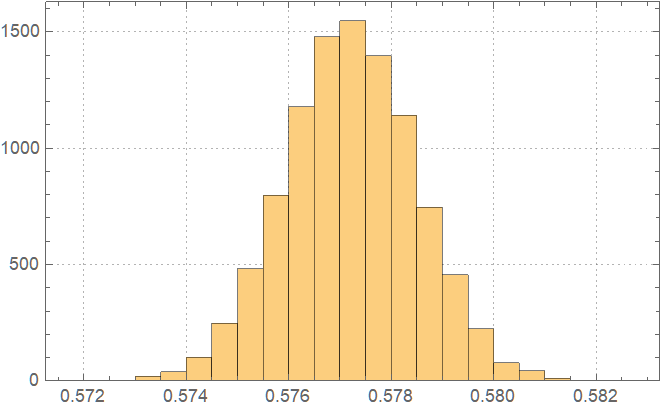
\includegraphics[width=10cm]{Images/repeatedgamma.png}
    \caption{Histogram of experiment with $10^6$ points, repeated $10^4$ times.}
    \label{fig:repeatedgamma}
\end{figure}
\FloatBarrier
\subsection{Stieltjes constants}
Calculating Stieltjes constants is not a trivial task, there exist many infinite series representations of Stieltjes constants which converge very slowly \cite{stieltjeswolfram} (see eq.12). Extensive work has also been done in implementing fast algorithms to compute Stieltjes constants with high accuracy \cite{johansson2018computing}.
\par We will approximate a few Stieltjes constants by estimating the following integral definition.
\begin{align}
    \gamma_n = \frac{(-1)^n n!}{2 \pi} \int_0^{2 \pi} e^{nix} \zeta (e^{ix}+1)\, dx \label{5.4}
\end{align}
\par The above integral is derived by using Cauchy's differentiation formula on $$(-1)^n \gamma_n= \frac{d^n}{dz^n} \left. \left ( \zeta(z) - \frac{1}{z-1}\right)\right|_{z=1}$$
which is in turn obtained by comparing the Laurent series of the Zeta function with a traditional Taylor series.
\par The reader should note that calculating Stieltjes constants with Monte Carlo integration is not at all practical due to the low accuracy. For practical approximations other forms of numerical integration techniques are used \cite{johansson2018computing, newtoncotes}.
\par We will estimate eq. \ref{5.4} using the naïve Monte Carlo integration described in the first section. The following table shows the results we achieved.

\begin{table}[!htb]
\centering
\resizebox{\textwidth}{!}{%
\begin{tabular}{@{}cccccc@{}}
\toprule
$\gamma_n$ & \begin{tabular}[c]{@{}c@{}}No. of \\ points chosen\end{tabular} & \begin{tabular}[c]{@{}c@{}}No. of times \\ repeated\end{tabular} & \begin{tabular}[c]{@{}c@{}}Mean and\\ Standard Deviation\end{tabular} & Real values & Percentage Error \\ \midrule
$1$ & $10^5$ & $10^4$ & $-0.0728663 \pm 0.00258$ & $-0.0728159$ & $-2.00069 \cdot 10^{-2}$ \\
$2$ & $10^5$ & $10^4$ & $-0.00969426 \pm 0.00524$ & \multicolumn{1}{l}{$-0.0096904$} & $+4.02199 \cdot 10^{-2}$ \\
$3$ & $10^5$ & $1.5 \cdot 10^4$ & $+0.00204329 \pm 0.01551$ & $+0.0020538$ & $-5.13216 \cdot 10^{-1}$ \\
$4$ & $10^5$ & $3 \cdot 10^4$ & $+0.00233049 \pm 0.06136$ & \multicolumn{1}{l}{$+0.0023253$} & $+2.20283 \cdot 10^{-1}$ \\ \bottomrule
\end{tabular}%
}
\caption{Computed values of the first 4 Stieltjes constants (not including 0)}
\label{tab:stieltjescal}
\end{table}
\begin{figure}[!htb]
    \centering
    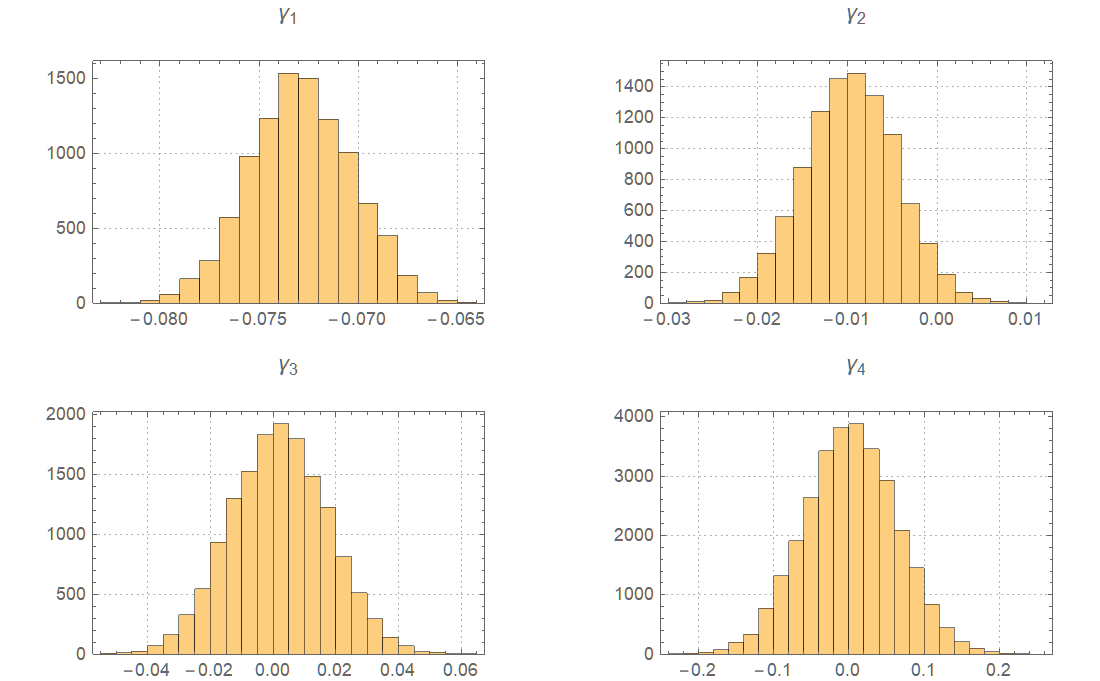
\includegraphics[width=\textwidth]{Images/stieltjesconstantsgrid.png}
    \caption{Histogram of the 4 experiments.}
    \label{fig:repeatedstieltjes}
\end{figure}
\clearpage
% --------------------------------------------------------------------------------
%	Section 6
%----------------------------------------------------------------------------------------
\section{Estimating Phi}
We conclude the estimation of mathematical constants on a lighter note.
\par Since the golden ratio ($\varphi$) is an algebraic number, estimating $\varphi$ is very trivial. Since we know that $\varphi = \frac{1+\sqrt{5}}{2}$, we can simply choose an integral which evaluates to the desired result. We will choose $\int_4^5 \frac{3}{2}+\frac{1}{4 \sqrt{x}}\ dx$ which is evidently equal to $\varphi$.
\par We estimate the integral with the method described in Section 1.
\par We repeat the experiment $10^4$ times with $10^6$ points per experiment. Taking the mean of these $10^4$ experiments gives us the following approximation, $\varphi \approx 1.61803 \pm 3.79948 \cdot 10^-6$, with $6.544 \cdot 10^{-7}\ \%$ error. In fact the approximation is correct up to 7 decimal places!
\begin{figure}[!htb]
    \centering
    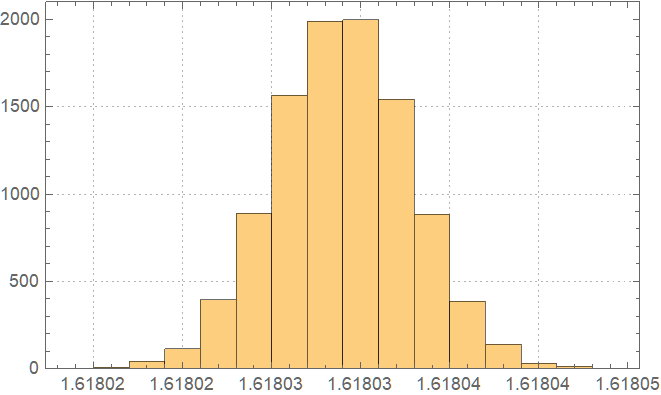
\includegraphics[width=10cm]{Images/repeatedphi.png}
    \caption{Histogram of experiment with $10^6$ points, repeated $10^4$ times.}
    \label{fig:repeatedphi}
\end{figure}
%----------------------------------------------------------------------------------------
%	Section 7
%----------------------------------------------------------------------------------------
\section{Methods of integral variance reduction}
Throughout the project so far we have only considered what is known as "naïve" Monte Carlo integration. We will now justify its nomenclature by listing out a few modified methods of Monte Carlo integration that are so designed to reduce variability \cite{caflisch_1998, anithetic}.
\par To demonstrate the effectiveness of these method we will be estimating the following integral,
\begin{align}
    \int_0^1 \int_0^1 \frac{\sin x \sin y}{x y}\, dx\, dy \label{sinx}
\end{align}
\par
It is a well known fact that $\int_0^z \frac{\sin x}{x}\, dx$ has no elementary closed form, in fact it is just represented by $Si(z)$ for simplicity. It is then clear to see that eq. \ref{sinx} is equal to $Si(1)^2$.
\subsection{Antithetic variates}
Antithetic variates is a technique for variance reduction, in which we use the antithetic pair ($-x_1, \cdots, -x_n$) of pre-obtained samples ($x_1, \cdots x_n$) in the Monte Carlo simulation.
The advantage of this technique is that, it reduces the number of
% normal 
samples to be taken to generate $N$ integration nodes, and thus, reduces the variance of the sample 
\par We will give a short proof of the above statement.
\begin{theorem}
Random variable X and Y, on the same probability space are antithetic if they have same distribution and their covariance is negative. 
\end{theorem}

   Take two variable X and Y . the variance of the average of $x,y$ is 
   \begin{align*}
       \text{Var}\left[\frac{1}{2}(x+y)\right]&=\frac{1}{4}[\text{Var}(X) + \text{Var}(Y)+2 \text{ Cov}(X,Y)]
       \intertext{since we know that,}
       \text{Cov}(X,Y)&=\rho \sqrt{\text{Var}X}\sqrt{\text{Var}Y}
       \shortintertext{where $\rho$ is the correlation between X and Y. It can be clearly seen that Var(X+Y) is minimised when $\rho=-1$ i.e if X and Y are perfectly negatively correlated.} \QED
   \end{align*}
  Now we will compare antithetic variables vs naïve Monte Carlo with eq. \ref{sinx}.
\begin{figure}[!htb]
    \centering
    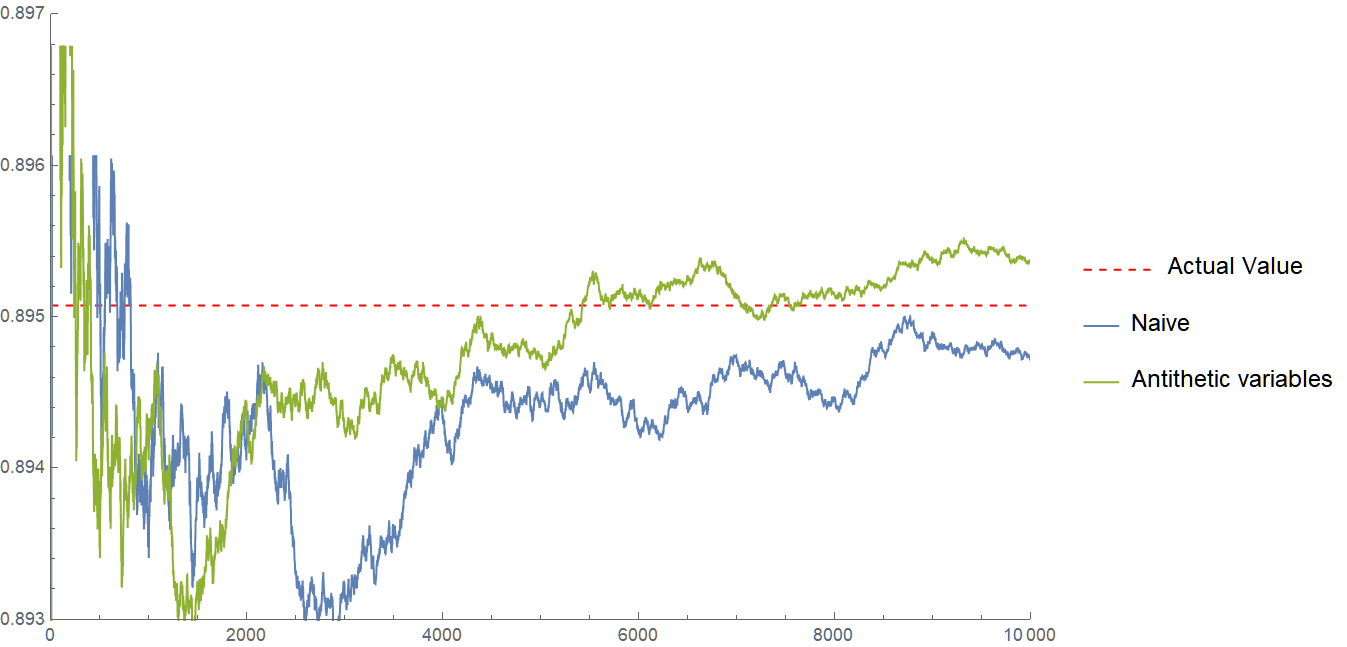
\includegraphics[width=13cm]{Images/naivevsanti.png}
    \caption{Comparison of estimating e.q. \ref{sinx} with naïve Monte Carlo vs Monte Carlo with antithetic variables (for points ranging from 1 to 10,000).}
    \label{fig:naivevsanti}
\end{figure}
\subsection{Control variates}
\par In this variance reduction technique, we use a known integral with a value approximately equal to the unknown integral to reduce the error in the estimate of unknown integral.
\begin{theorem}
$I[f] \approx \frac{1}{N} \sum_{i=1}^N (f(X_i)-g(X_i)) + \theta$
\end{theorem}
Suppose we want to find $\mu= E[f(x)]$. We find some $\theta=E[g(x)]$ where $g(x)\approx f(x)$,
hence $\widehat{\mu}=\frac{1}{N}\sum_{i=1}^N f(X_i)$ and $\widehat{\theta}=\frac{1}{N}\sum_{i=1}^N g(X_i)$ for a r.v. $X$. We can estimate $\mu$ by the following estimator,
\begin{align*}
\widehat{\mu}_{\text{diff}}=\frac{1}{N}\sum_{i=1}^N (f(x_i)-g(x_i))+\theta
\end{align*}
\par This estimator is motivated due to the linearity of integrals.
The expected value of $\widehat{\mu}=\mu$, since $E[\widehat{\theta}]=\theta$. 
\begin{align*}
    \text{Var}(\widehat{\mu}_{\text{diff}}) =\frac{1}{N} \text{Var} ( f(X) -g(X))
    \intertext{If $f(X)\approx g(X)$, then,}
    \text{Var} (f(X) - g(X)) < \text{Var}(f(X)) 
    \shortintertext{Hence, we use $(\widehat{\mu}_{\text{diff}})$ to reduce the variance. Here $g(X)$ is known as the control variate.} \QED
\end{align*}

\par We will now compare Monte Carlo integration in estimating eq. \ref{sinx} using both control variates as well as antithetic variables.
\par To generate a known integral $g(x)$ which is close to $f(x)$ we will employ the use of taylor series. Finding the taylor series of $f(x)$ about $0$, we estimate the integrand as follows,
\begin{align*}
    \frac{\sin x \sin y}{xy}&=\sum _{n=0}^\infty \sum _{m=0}^\infty x^n y^m \frac{\cos \frac{m \pi}{2} \cos \frac{n \pi}{2}}{ (m+1)! (n+1)!}
    \intertext{Using n=m=0 to n=m=2 as a approximation we get,}
    \frac{\sin x \sin y}{xy}&\approx 1-\frac{x^2}{6}-\frac{y^2}{6}+\frac{x^2 y^2}{36}
\end{align*}
We therefore use this approximation as $g(x)$,
\begin{align}
    g(x)&=\int_0^1 \int_0^1 1-\frac{x^2}{6}-\frac{y^2}{6}+\frac{x^2 y^2}{36}\, dx\, dy= \frac{289}{324}
\end{align}
\par Finding a taylor series is obviously not practical for most integrands, but even very rough approximations will significantly reduce variability.

\begin{figure}[!htb]
    \centering
    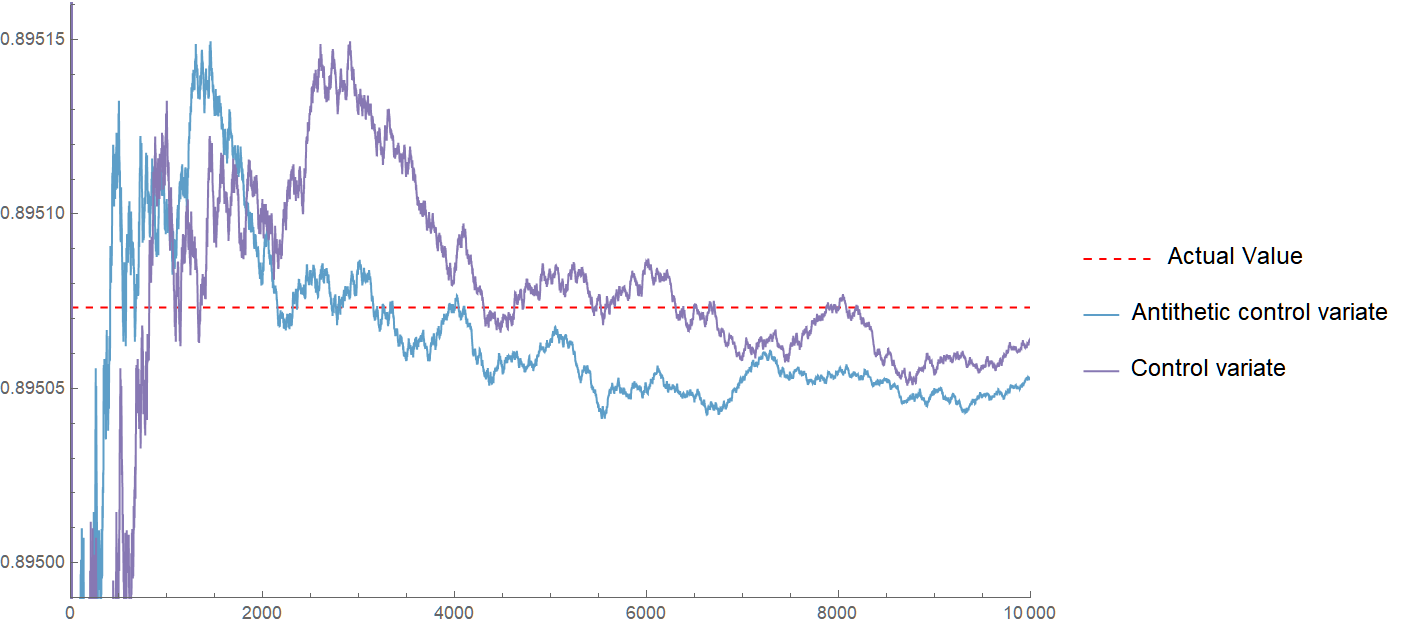
\includegraphics[width=\textwidth]{Images/controlvariate.png}
    \caption{Comparison of estimating e.q. \ref{sinx} with control variate Monte Carlo vs Monte Carlo with antithetic variables and control variate (for points ranging from 1 to 10,000).}
    \label{fig:controlvariate}
\end{figure}
\FloatBarrier
\par To put this the effectiveness of the control variate method in perspective we shall see it in comparison to the naïve method.

\begin{figure}[!htb]
    \centering
    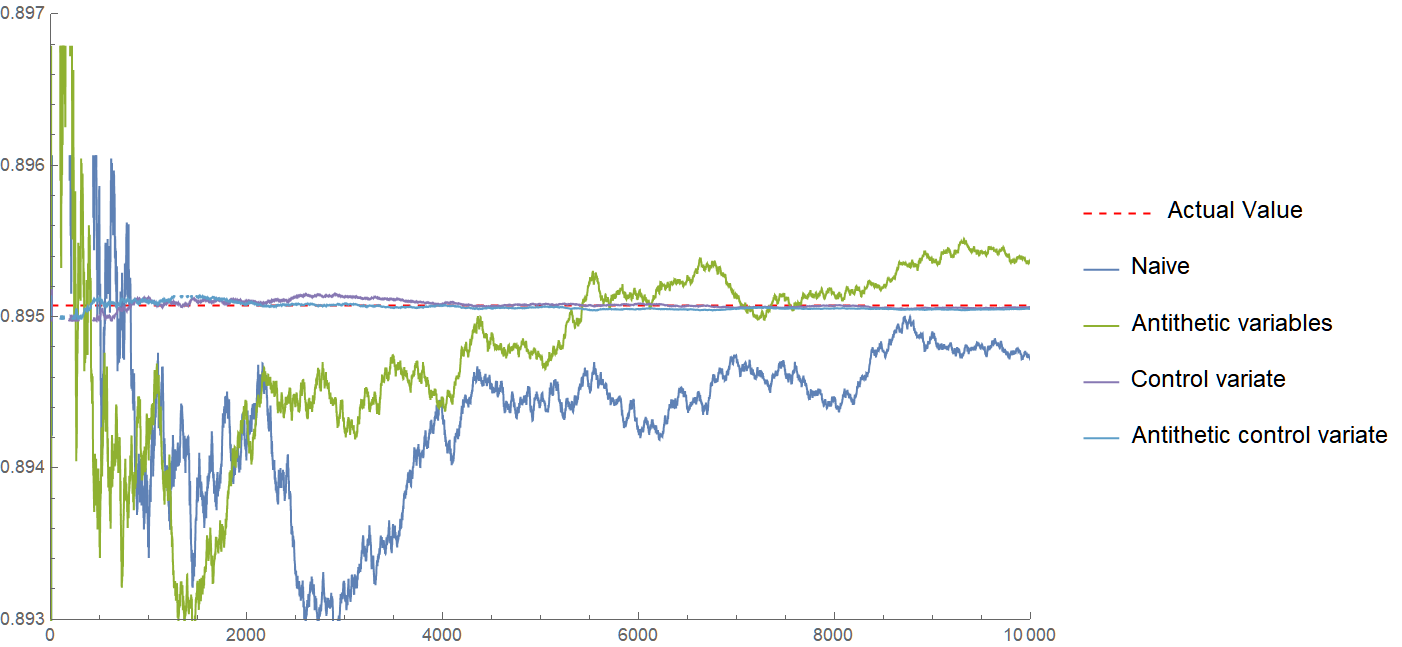
\includegraphics[width=\textwidth]{Images/controlvsnaiveanti.png}
    \caption{Comparison of the control variate with naïve Monte Carlo.}
    \label{fig:controlvsnaivevariate}
\end{figure}
\par The reduction is variance is now much more striking.

\clearpage
\section{Quasi Monte-Carlo integration}
Quasi-Monte Carlo integration, simply put, is Monte Carlo integration using quasi-random generated numbers to form the integration nodes (as opposed to pseudo-random in naïve integration) \cite{MOROKOFF1995218}.
\par The reader should note that in this section, we will only provide a cursory overview of Quasi Monte-Carlo integration and its results. Detailed proofs will not be given as they are far beyond the scope of this project. A vast amount of the theory surrounding this topic has been carried out by H. Niederreiter in a series of papers \cite{Niederreiter1978QuasiMonteCM, lowdiscrepancyNIEDERREITER198851} and books \cite{kuipers1974uniform} which we recommend for further reading.
\subsection{Quasi-random sequences (low-discrepancy sequences)}
\par Quasi-random numbers are numbers generated from quasi-random sequences, which are in turn defined as sequences with low discrepancy \cite{quasirandomdiscrepancy}. We will first define what is meant by discrepancy.
\par
Discrepancy can be intuitively thought of as a measure of uniformity. We will now see the formal definition for discrepancy for a one-dimensional sequence \cite{Niederreiter1978QuasiMonteCM}.
\par Let $x_1, x_2, \cdots x_N$ be $N$ numbers in $I=[0,1]$, let $E \subset I$. Define a function $A(E;N)$ such that, it counts the number of $n, 1\leq n\leq N$, for $x_n \in E.$ The discrepancy $D_n$ of the $N$ numbers in $I$ is then given by,
\begin{align}
    D_n=\sup_J \left| \frac{A(J;N)}{N}-|J| \right|
    \intertext{Where, $J$ is any sub-interval of $I$. The star discrepancy ($D_N^*$) is a more commonly used definition which is as follows.}
    D_N^*=\sup_{0\leq t \leq 1} \left | \frac{A([0,t); N)}{N} - t  \right|
\end{align}
\par These above definitions are easily generalized to $[0,1]^s$ by calculating $|J|$ with the respective metric.
\par $D_n$ and $D_n^*$ are related by the following inequality \cite{Niederreiter1978QuasiMonteCM}
\begin{align}
    D_n^* \leq D_n \leq 2^s D_n^* \label{starrelation}
\end{align}
\clearpage
\subsection{Error in Quasi Monte-Carlo integration}
Niederreiter has shown \cite{Niederreiter1978QuasiMonteCM} that for any dimension $s \geq 1$, there exists an infinite sequence of points in $I^s$ such that, for some constant $c_s$ only dependent on dimension, 
\begin{align*}
    D_N = O \left(c_s \frac{\log N ^s}{N}\right)
\end{align*}
The famous Koksma–Hlawka inequality states that \cite{Niederreiter1978QuasiMonteCM},
\begin{align*}
    \left| \frac{1}{N} \sum_{n=1}^{N} f(x_n)-\int_{[0,1]^s} f(x) dx \right| \leq V(f) D_N^*
\end{align*}
Where, $V(f)$ is the bounded total variation of the function \footnote{Note that this is not variance. Discussing total variation rigorously is well beyond the scope of this project, it can be roughly thought of as a infinitesimal absolute value.}.
\par The Koksma-Hlawka inequality along with eq. \ref{starrelation} is used to show that the error of Quasi Monte-Carlo integration is given by $O \left(c_s \frac{\log N ^s}{N}\right)$ as opposed to $O \left(\frac{1}{\sqrt{N}}\right)$ when using random numbers.
\par It is then clear to see that for a sufficiently small dimension $s$ and $c_s$ the error by Quasi Monte-Carlo integration is much lower than naïve Monte-Carlo integration.
\subsection{Examples of Quasi-Random sequences}
We have so far restrained from giving any examples of methods used to generate quasi-random sequences. In this section we will describe a few important methods \footnote{We will not be proving the values of discrepancies of these examples.}.
\subsubsection{Van der Corput and Halton sequence}
We begin by describing Van der Corput sequences \cite{kuipers1974uniform}, which are conceptually the easiest to understand. 
\par For any integer $n\geq 0$ as follows, we define the following function, known as the radical-inverse function,
\begin{align}
    \phi_b(n)=\sum_{j=1}^m a_j b^{-j}=\frac{a_1}{b}+\frac{a_2}{b^2}\cdots \label{radicalinverse}
\end{align}
for $a_j$ ranging 0 to $b-1$, $m, b\in \mathbb{Z}$ and $b \geq 2$. The reader should note the similarity of this function with the base $b$ representation of a number. $\phi_b(n)$ is clearly contained in $[0,1]$.
\par The Van der Corput sequence is defined for any range of $n$'s as,
\begin{align}
    x_n=\phi_2(n)
\end{align}
With star discrepancy equal to,
\begin{align}
    D_N^*= O \left( \frac{\log N}{N}\right)
\end{align}
Below we enumerate the first 5 values of the Van der Corput sequence.
\begin{table}[h!]
\centering
\begin{tabular}{ccc}
\hline
$n$ & $n_2$ & $\phi_2(n)$ \\ \hline
$0$ & $0$ & $0$ \\
$1$ & $1$ & $0.1_2=1/2_{10}$ \\
$2$ & $10$ & $0.01_2=1/4_{10}$ \\
$3$ & $11$ & $0.11_2=3/4_{10}$ \\
$4$ & $100$ & $0.001_2=1/8_{10}$ \\ \hline
\end{tabular}
\caption{First 5 values of Van der Corput sequence}
\label{tab:vandercorput}
\end{table}
\par 
However, the limitation of Van der Corput should now be clear to see. Van der Corput sequences only generates single dimensional numbers.
\par Halton sequences \cite{halton} are a very natural extension of Van der Corput sequences for higher dimensions $s$, which we define as,
\begin{align}
    x_n^s=(\phi_{p_1}(n), \phi_{p_2} (n), \cdots,\phi_{p_s}(n))
\end{align}
Where, $p_1, p_2 \cdots p_s$ must are co-prime integers. It is common to simply use the $n^{th}$ prime number at each stage. The reason for this specific selection of bases is to reduce the dimension dependent constant in the discrepancy.
\par The star discrepancy of Halton sequences is, as expected,
\begin{align}
    D_N^*= O \left( \frac{\log N^s}{N}\right)
\end{align}
It has been theorized that Van der Corput and Halton sequences have the lowest discrepancy of any quasi-random sequence. This is however not yet been proved. Nevertheless, Halton sequences are very rarely used for numeric integration  due to its tendency of becoming overly predictable in higher dimensions.
\par An early fix for this problem was given by Faure \cite{faure} who proposed to use bases in the Halton sequence as the first prime number greater than dimension $s$, and further to re-order each element using certain permutations based on Pascal matrices.
\par Below we have displayed a 2-dimensional Halton sequence with 1500 points using base 2 and 3. To illustrate the predictable nature for high dimensions we will also display a 2-dimensional graph using the 10th and 11th prime respectively.
\begin{figure}[!htb]
    \centering
    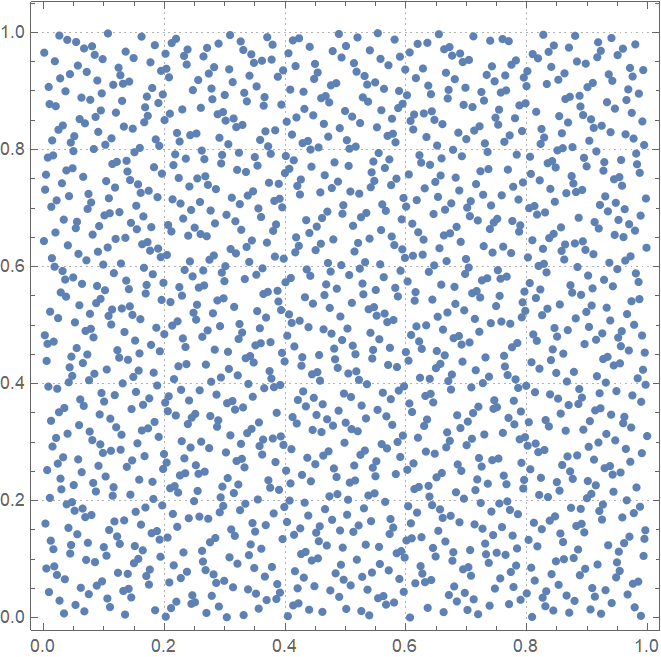
\includegraphics[width=8cm]{Images/23halton.png}
    \caption{2-D Halton sequence with 1500 points using $2^{nd}$ and $3^{rd}$ prime as bases.}
    \label{fig:example23halton}
\end{figure}
\begin{figure}[!htb]
    \centering
    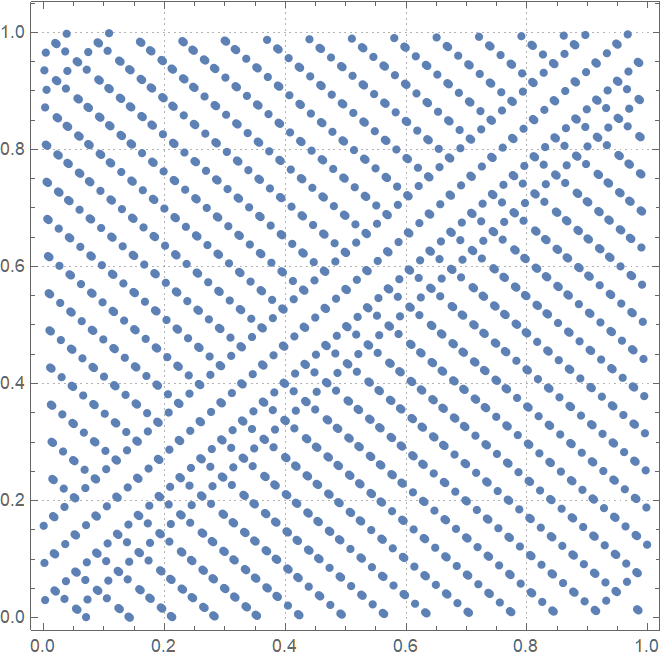
\includegraphics[width=8cm]{Images/1011halton.png}
    \caption{2-D Halton sequence with 1500 points using $10^{th}$ and $11^{th}$ prime as bases. This helps visualize the problem of overly predictive points that occur in higher dimensions.}
    \label{fig:example1011halton}
\end{figure}
\clearpage
\subsubsection{A cursory view of (t,s) sequences}

Before expounding on a few other types of quasi-random sequences (namely, Sobol and Niederreiter) we will first list out a few important definitions in a summarized manner. Throughout this section we will extensively refer to a paper by J. Dick and H. Niederreiter \cite{exactnied}.
\par Recall the definition of the radical-inverse function (see e.q. \ref{radicalinverse}). For some $\mathbf{x} \in [0,1]^s$ consider, $$[\mathbf{x}]_{b, m}=(\phi_b(x^1), \cdots, \phi_b(x^s))$$ Here $m$ is the upper bound of summation. Note the difference between the Halton sequence, here we use a fixed base $b$.
\par For integers $b\geq 2, s\geq 1$ and $t \geq 0$. Consider a sequence of points $x_0, x_1, \cdots$, in $[0,1]^s$. This sequence of points is called a \textbf{\textit{(t, s)} sequence} in base $b$. If for all integers $k\geq0$ and $m > t$, the set $\mathcal{P}_{k,m}$ consisting of the points $[x_n]_{b,m}$ with $kb^m \leq n < (k+1)b^m$ has the following property-
\\
\textit{for every half-open sub-interval $E$ of $[0,1]^s$ of the following form}
\begin{align}
    E= \prod_{i=1}^s [a_i b^{-c_i}, (a_i+1)b^{-c_i}) \label{elementary}
\end{align}
\par \textit{for some integers $c_i>0$ and $0\leq a_i < b^{c_i}$ for $1\leq i \leq s$ and volume $b^{t-m}$,}\\
there are exactly $b^t$ points of $\mathcal{P}_{k,m}$ contained in E.
\par For the purposes of this project we are not providing detailed motivation for the concept of (t,s) sequences, we state it in a simplified definition since both Niederreiter and Sobol sequences are in fact (t,s) sequences.
\subsubsection{Niederreiter sequence}
Niederreiter sequences are considered to be the best quasi-random sequence for numerical integration. Here we shall provide a very brief overview of Niederreiter sequences \cite{exactnied, lowdiscrepancyNIEDERREITER198851} without going into details of the construction, with an example at the end.
\par Consider for some fixed dimension $s\geq 1$, consider a list of pairwise co-prime non-constant polynomials belonging to any finite field of order $q$,\footnote{With the ordinary restriction that q is a power of some prime.} with $e_i=$ deg($p_i)\geq 1$ for $1 \leq i \leq s.$ , i.e., $p_1, p_2, \cdots p_s \in \mathbb{F}_q$.
\par The generating matrices for the Niederreiter sequence are constructed using the constants of the Laurent series expansions over these polynomials and objects known as (t,m,s) nets \footnote{We have refrained from defining (t,m,s) nets as we are not providing the full proof. They are closely related to (t,s) sequences.}.
\par For more detailed expositions refer to the papers by Niederreiter \cite{exactnied, tmsandtsnied,lowdiscrepancyNIEDERREITER198851}. The matter of note is that the Niederreiter sequences in fact form (t,s) sequences with the exact value of $t$ given as follows,
$$ t= \sum_{i=1}^{s}(e_i-1) $$
\begin{figure}[!htb]
    \centering
    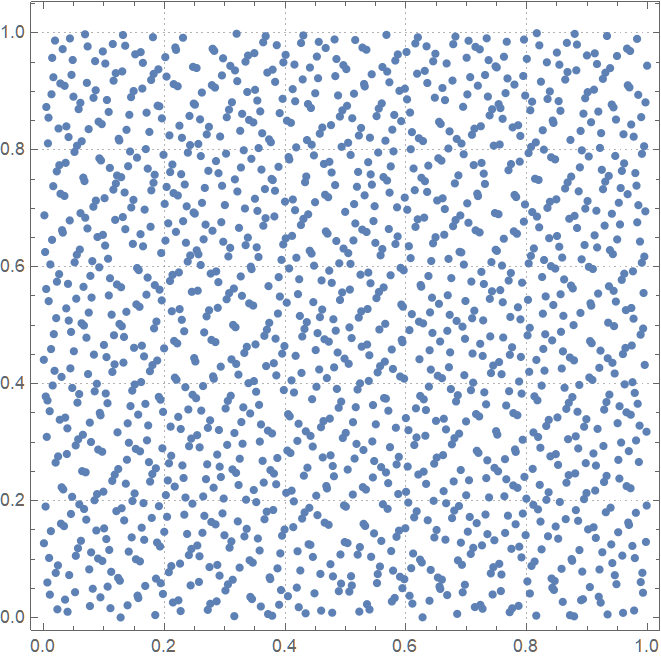
\includegraphics[width=8cm]{Images/1500neiederreiter.png}
    \caption{An example of a 2-Dimensional Niederreiter sequence with 1500 points.}
    \label{fig:examplenied}
\end{figure}
\subsubsection{Sobol sequence} 
Sobol sequences can be thought of as a special case of the Generalized Niederreiter sequence \cite{exactnied, SOBOL196786}. It also uses polynomials to generate the quasi-random sequence.
\par Sobol sequences can be thought of as a (t,s) sequences in base 2 that uses polynomials as such, $p_1(x)=x \in \mathbb{F}_2[x]$ and $p_2, \cdots, p_s$ being primitive polynomials of successive order arranged in non-decreasing degrees to construct the generating matrices.
\par Note the difference, Sobol uses primitive polynomials in base 2 while Niederreiter uses any pairwise co-prime polynomials in any base.
\begin{figure}[!htb]
    \centering
    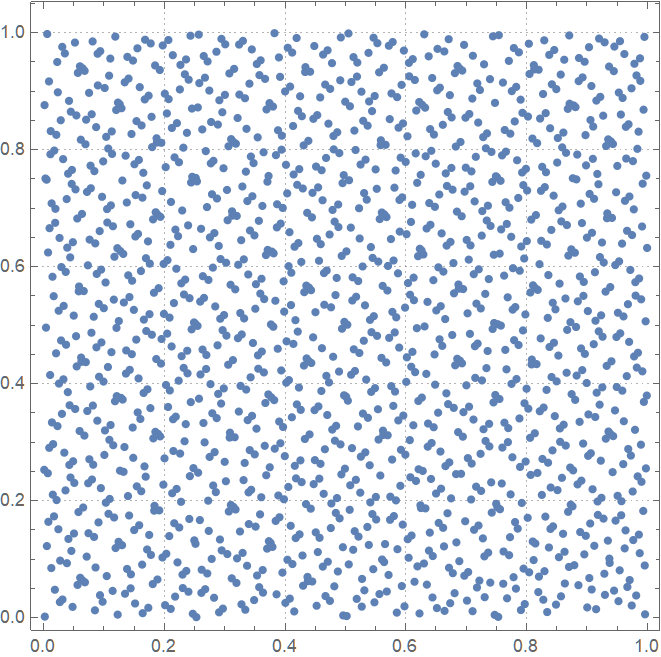
\includegraphics[width=8cm]{Images/1500sobol.png}
    \caption{An example of a 2-Dimensional Sobol sequence with 1500 points.}
    \label{fig:examplesobol}
\end{figure}
\FloatBarrier
\subsection{Computing Apery's constant}
We will end the project by computing a final example using Quasi Monte Carlo integration.\par
Apery's constant is $\zeta(3)=\sum_{n=0}^{\infty}\frac{1}{3^n}$. A simple integral representation of Apery's constant is given as follows,
\[\zeta(3)=\int_0^1\int_0^1\int_0^1 \frac{1}{1-xyz}\, dx\, dy\, dz\]
\par For comparisons sake we will estimate the integral with Quasi Monte-Carlo and naïve Monte Carlo to provide a direct comparison. This is shown in the graph below.
\begin{figure}[!htb]
    \centering
    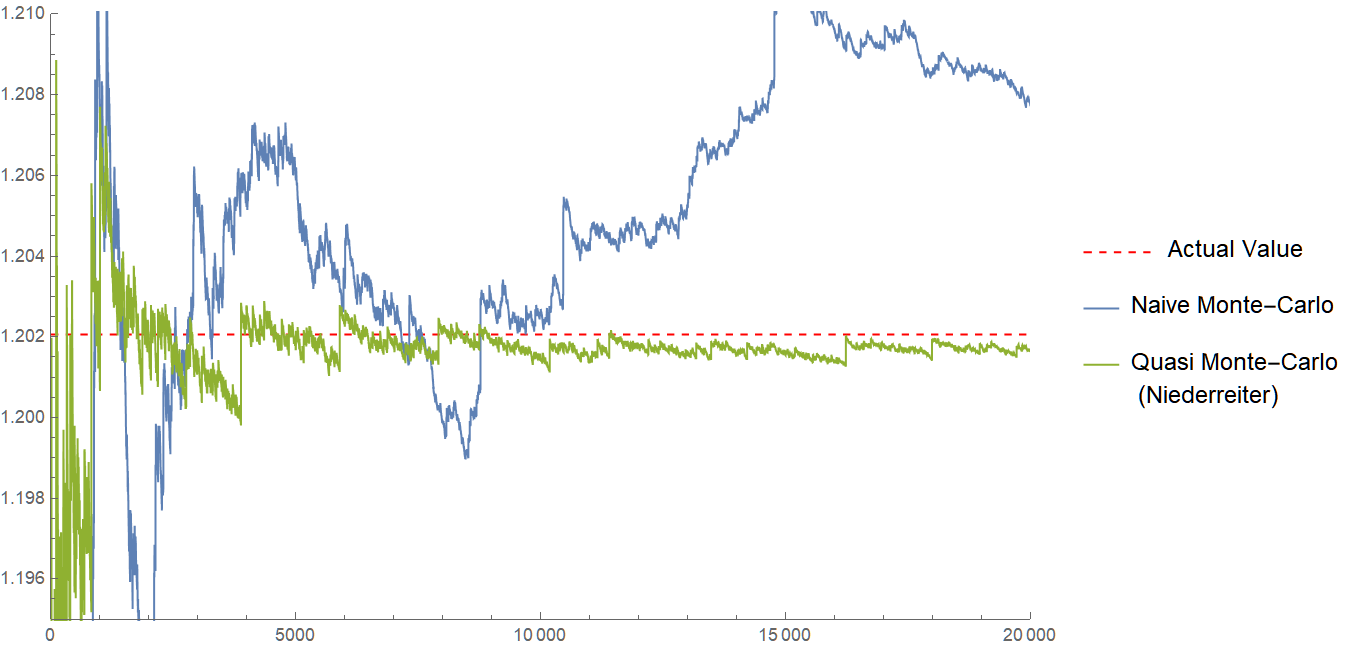
\includegraphics[width=\textwidth]{Images/aperyquasi.png}
    \caption{Quasi Monte Carlo vs naïve Monte Carlo estimates for Apery's constant (no. of points ranging from 1 to 20,000).}
    \label{fig:aperyquasi}
\end{figure}
\par Repeating the experiment using the Niederreiter sequence with $10^6$ points repeated $10^2$ times we obtain the following results.
\par $\zeta(3)\approx 1.202055 \pm 3.095 \cdot 10^{-5}$, with a percentage error of $-1.514 \cdot 10^{-4} \%.$
\FloatBarrier
\bibliographystyle{unsrt}
\bibliography{references}
\end{document}